\subsection{Verifica e validazione}
Il periodo di verifica e validazione ha inizio il xxdataxx e termina il xxdataxx.
Le attività svolte in questo periodo rappresentano la sintesi delle attività di verifica svolte lungo il corso del progetto.

\subsubsection{Incrementi}
Gli incrementi effettuati saranno 2, le principali attività svolte:
\begin{itemize}

	\item \textbf{Incremento e Verifica:} quest'attività prevede l'aggiornamento e la verifica di tutta la documentazione di progetto alla luce dei risultati della Revisione di Qualifica;

	\item \textbf{Validazione e Collaudo:} quest'attività prevede la validazione del prodotto al fine di assicurarsi e dimostrare che sia conforme alle specifiche del cliente;

\end{itemize}
 
 \subsubsection{Verifica e validazione - Gantt delle attività}

\begin{figure} [H]
	\centering
	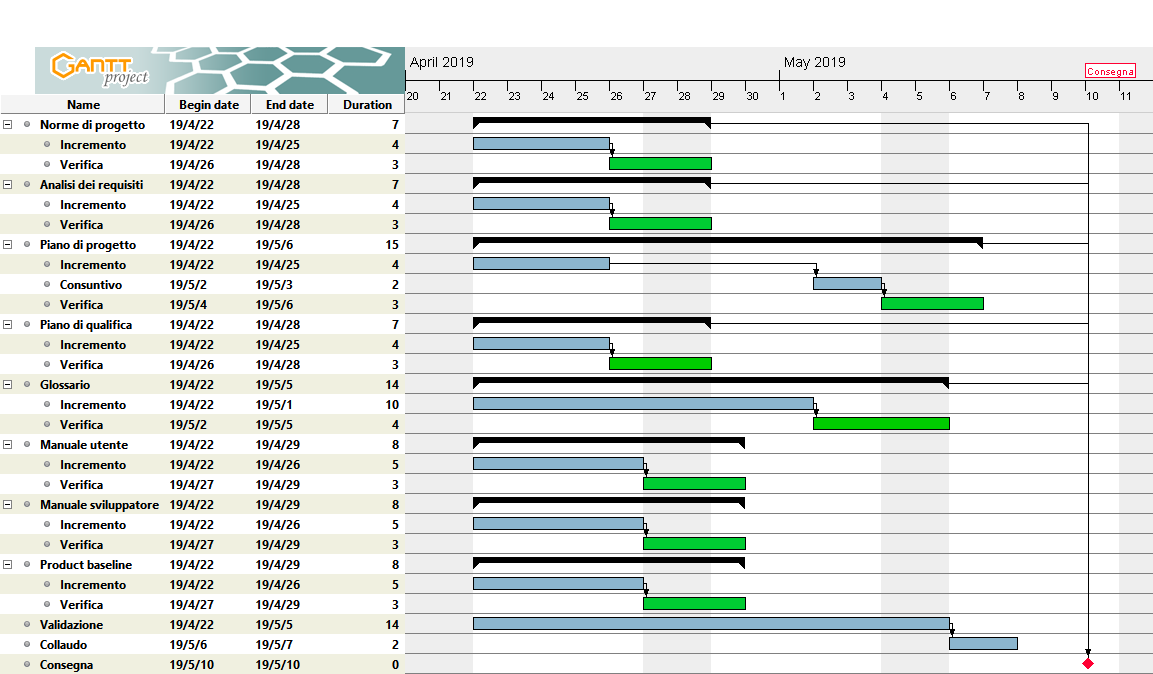
\includegraphics[scale=0.35]{Res/Gantt/Validazione}
	\caption{Figura 4.5: Diagramma di Gantt del periodo "Verifica e validazione"}\label{}
\end{figure}

 
\pagebreak
